% Chapter 3

\chapter{Methodology} % Write in your own chapter title
\label{Chapter3}
\lhead{Chapter 3. \emph{Approach of Weather Classification}}

\section{Dataset}

There are over 15 million labelled images in the ImageNet database which has 22,000 categories. The images were collected from the Internet and labelled manually. From 2010, the competition, named the ImageNet Large-Scale Visual Recognition Challenge(ILSVRC) \citep{deng2009imagenet}, has been held annually. The competition uses a subset of dataset which contains 1000 images in 1000 categories. With 50,000 validation images and 150,000 testing images, there are over 1 million images in total.
\graphicspath{ {./Figures/} }
\begin{figure}[!htb]
    \centering
	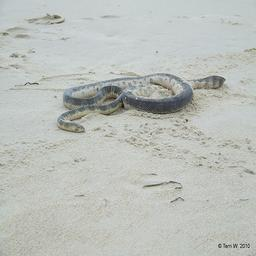
\includegraphics[width=0.4\textwidth]{ILSVRC2012_val_00000001.JPEG}
    \qquad
    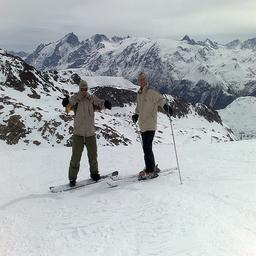
\includegraphics[width=0.4\textwidth]{ILSVRC2012_val_00000002.JPEG}
    \caption{2 Figures from the ImageNet \citep{deng2009imagenet}.}%
    \label{fig:ImageNetExamples}%
\end{figure}

The weather dataset \citep{lutwo} contains 10,000 images for two categories evenly, cloudy and sunny. They were collected from three sources, the Sun Dataset \citep{russell2008labelme}, the Labelme Dataset \citep{xiao2010sun} and the website, Flickr. They were classified manually and similar images were removed. No unambiguous images exist in the dataset.
\graphicspath{ {./Figures/} }
\begin{figure}[!htb]
    \centering
	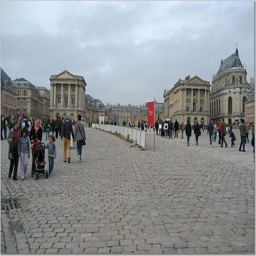
\includegraphics[width=0.4\textwidth]{cloudy_0001.png}
    \qquad
    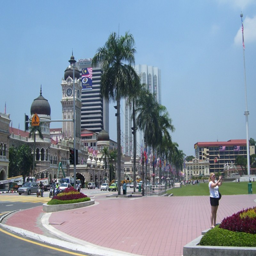
\includegraphics[width=0.4\textwidth]{sunny_0003.png}
    \caption{2 Figures from the Weather Dataset \citep{lutwo}.}%
    \label{fig:WeatherExamples}%
\end{figure}

In general, the two datasets are different. The ImageNet dataset is used for object classification and the weather dataset is used for scene classification. The objects of the images are different too. Because the images, of the two datasets, are different size, we have to resize them to a fixed $224 \times 224$ to feed into CNN.

\section{Data Argumentation}

\graphicspath{ {./Figures/} }
\begin{figure}[!htb]
    \centering
    \subfigure[original image]{
		\begin{minipage}{0.3\textwidth}
		   		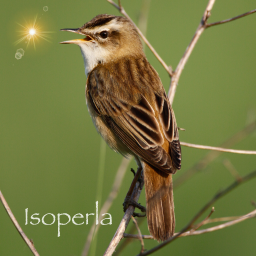
\includegraphics[width=1\textwidth]{crop}
		   		\label{fig:orig}
		\end{minipage}
    	} 
    \subfigure[cropped from left up]{
		\begin{minipage}{0.3\textwidth}
		   		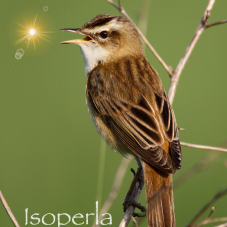
\includegraphics[width=1\textwidth]{cropleftup}
		   		\label{fig:leftup}
		\end{minipage}
    	} 
    \subfigure[cropped from left down]{
		\begin{minipage}{0.3\textwidth}
		   		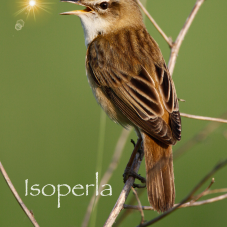
\includegraphics[width=1\textwidth]{cropleftdown}
		   		\label{fig:leftdown}
		\end{minipage}
    	} 
    \subfigure[cropped from right up]{
		\begin{minipage}{0.3\textwidth}
		   		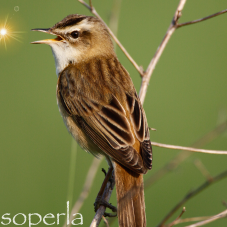
\includegraphics[width=1\textwidth]{croprightup}
		   		\label{fig:rightup}
		\end{minipage}
    	} 
    \subfigure[cropped from right down]{
		\begin{minipage}{0.3\textwidth}
		   		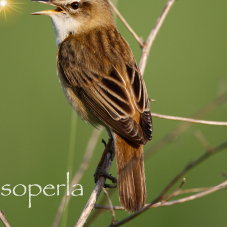
\includegraphics[width=1\textwidth]{croprightdown}
		   		\label{fig:rightdown}
		\end{minipage}
    	} 
    \subfigure[cropped from center]{
		\begin{minipage}{0.3\textwidth}
		   		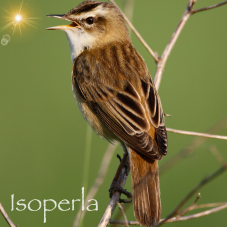
\includegraphics[width=1\textwidth]{cropcen}
		   		\label{fig:cropcen}
		\end{minipage}
    	} 

    \caption{A set of cropped patches from original image}%

    \label{fig:dataargument}%
\end{figure}
The CNN architecture \citep{krizhevsky2012imagenet} has about 60 million parameters, and it is essential to avoid overfitting. One of methods is data argumentation. The dataset is artificially enlarged by cropping and horizontal reflecting images. For each $256\times256$ image, the network extracts five $224\times224$ patches from four corners and center and reflects them horizontally. Hence, there are 10 patches extracted from $1$ image in total. Figures \ref{fig:dataargument} shows the method of data argumentation.
% add image examples here

\section{Spatial Pyramid Pooling (SPP)}

The factors, which have effects on scene classification, can be at any spatial position in an image. This could be a problem to CNN, because it was built up to recognise the objects in the center of images. The SPP layer can help to solve the problem.

The SPP layer is deployed behind the fifth convolutional layer. A set of bins are set to discern different local information from the output of the fifth convolutional layer. Assuming dimensions of feature maps are $a\times a$ and the bin size is $n$, each window size is $\lceil a/n \rceil$ and stride size is $\lfloor a/n \rfloor$, where $\lceil\,\rceil$ and $\lfloor\,\rfloor$ denote the ceiling and flooring operations. For the $l$ level pyramid, there are $l$ SPP layers. The layers will be concatenated into a fully connected layer. The bin sizes can be set to 1, 2, 3 and 6 for the SPP layers.

\begin{figure}[htb]
    \centering
	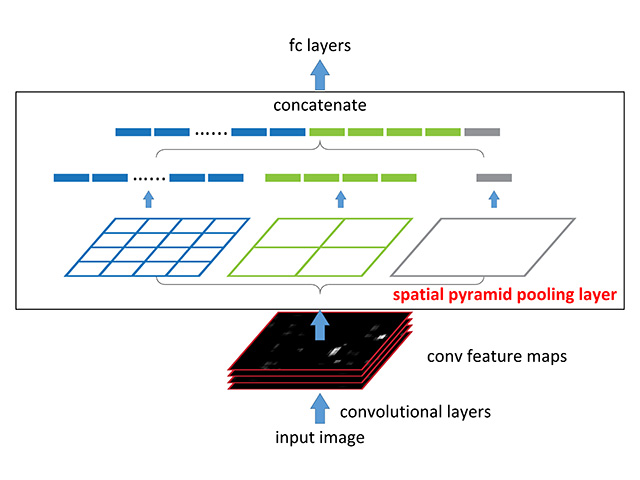
\includegraphics[width=0.8\textwidth]{sppnet.jpg}
    \caption{Diagram of the SPP layer \citep{he2014spatial}}%
    \label{fig:sppnet}%
\end{figure}

With the help of the SPP layer, most factors, in different scales, are taken into account.

\section{Convolutional Neural Networks Architecture}

Due to the significant performance of the AlexNet \citep{krizhevsky2012imagenet} which is a deep neural network, we train a model based on the network architecture. The architecture of the network has seven hidden adaptive layers, which are five convolutional layers and two fully connected layers.
\begin{figure}[htb]
    \centering
	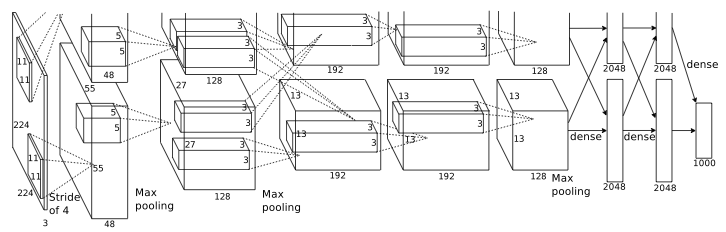
\includegraphics[width=0.8\textwidth]{AlexNet.png}
    \caption{Architecture of the AlexNet \citep{krizhevsky2012imagenet}}%
    \label{fig:ImageNetArch}%
\end{figure}
The network is very deep and has a huge number of parameters. It was implemented on two GPUs in the original experiment. The model is able to reach $62.5\%$ accuracy rates with one prediction and $83\%$ accuracy rates with five predictions in the competition.

The network use the ReLU \citep{nair2010rectified} as the activation function, which can achieve a faster learning speed than the $tanh$ function does. 

In the network, there are three types of layers and they play different roles in the model. The input data dimension is $224\times224\times3$. In the first convolutional layer, there are 98 kernels with size $11\times11$. The stride size is 4 and the outputs are 96 neurons. A following max pooling layer downsamples the spatial dimension. The second one filters the output of the previous pooling layer by $256$ kernels which size is $5\times5$. The third one owns 384 kernels with size $3\times3$. The fourth one has 384 kernels with size $3\times3$ and the last one has 256 kernels with size $3\times3$. After the convolutional layers, two fully connected layers have 4096 neurons each. At the end of network, there is a softmax layer with 1000 outputs.
\begin{table}[h]
\begin{center}
    \begin{tabular}{ | c | p{8cm} | }
    \hline
    Layer Name & Layer Description \\ \hline
    Input & 224 $\times$ 224 RGB image \\ \hline
    CONV1 & 11 $\times$ 11 conv, 96 ReLU neurons, stride 4 \\ \hline
    POOL1 & 3 $\times$ 3 max pooling, stride 2 \\ \hline
    CONV2 & 5 $\times$ 5 conv 256 ReLU neurons, stride 1 \\ \hline
    POOL2 & 3 $\times$ 3 max pooling, stride 2 \\ \hline
    CONV3 & 3 $\times$ 3 conv 384 ReLU neurons, stride 1 \\ \hline
    CONV4 & 3 $\times$ 3 conv 384 ReLU neurons, stride 1 \\ \hline
    CONV5 & 3 $\times$ 3 conv 256 ReLU neurons, stride 1 \\ \hline
    POOL5 & 3 $\times$ 3 max pooling, stride 2 \\ \hline
    SPP & bin size 1,2,3,6 \\ \hline
    FC6 & fully connect, ReLU 4096 neurons\\ \hline
    FC7 & fully connect, ReLU 4096 neurons\\ \hline
    FC8 & fully connect, ReLU 1000 neurons\\ \hline
    SOFTMAX & 1000 way softmax\\ \hline
    \end{tabular}
    \caption{Architecture of the model}
    \label{fig:NetPara}
\end{center}
\end{table}

















